\documentclass{scrartcl}
\usepackage[mathletters]{ucs}
\usepackage[utf8x]{inputenc}
\usepackage{amssymb}
\usepackage{amsmath}
\usepackage[usenames]{color}
\usepackage{hyperref}
\usepackage{wasysym}
\usepackage{graphicx}
\usepackage[normalem]{ulem}
\usepackage{enumerate}

\usepackage{listings}

\lstset{ %
basicstyle=\footnotesize,       % the size of the fonts that are used for the code
showspaces=false,               % show spaces adding particular underscores
showstringspaces=false,         % underline spaces within strings
showtabs=false,                 % show tabs within strings adding particular underscores
frame=single,                   % adds a frame around the code
tabsize=2,                      % sets default tabsize to 2 spaces
breaklines=true,                % sets automatic line breaking
breakatwhitespace=false,        % sets if automatic breaks should only happen at whitespace
}


\title{2 Spaghetti dataset}
\date{dinsdag 08 december 2020}
\author{}

\begin{document}

\maketitle

		\section{2 Spaghetti dataset}

Created vrijdag 04 december 2020



After the \href{./1_Birthday_dataset.tex}{Birthday dataset} a new dataset was created using the things learned from that. Now the amount of leds driven is reduced to 5 leds. Where led 6 to 11 is used to lighten the inserts. 

only the colors white and red are used for this dataset. This was discussed thad the red color could have an influence on the reflection of the carbide of which the inserts are made see \href{../../../../Research/Light/Light_Reflection.tex}{light reflection.}



\subsection{Dataset explanation}

For every insert, two pictures are taken. One with leds 6 to 11 on red and one with these leds white. This was experimentally found to be the best setting for reflecting the light off the worn area and into the camera. 

Turning on a led to much on the upper bounary will lighten the side of the insert which isn't of much use in this paper. Turining on a led to much on the bottom boundary makes the background very bright which supports unnessesary information.



The images are separated in a folder for every insert named with batch number and insert number:

batch\_aaa\_plate\_bbb where aaa is the batch number and bbb is the insert number.

Images are named with their settings, batch number and insert number:

b\_aaa\_p\_bbb\_l\_006-011\_color\_bullet.png 

where 

\begin{itemize}
\item aaa is the batch number; 
\item bbb is the plate number, 
\item 006-011 are the leds that turned on at the same time; 
\item color is the color: red or white
\item bullet is the appearance of a bullet on the side of the inset and has values of b for bullet or nb for no bullet.
\end{itemize}


The dataset inserts consisted of a few different types and coatings. 



\subsection{Setup}

The setup used is exactly the same as on the Birthday dataset where the camera is positioned as much to the top as possible. This can be seen on the picture:

Here we can see the led strips are a little bit twisted and are positioned very close to each other. This made the reflection better and should result in beter outcome of the algorithm.



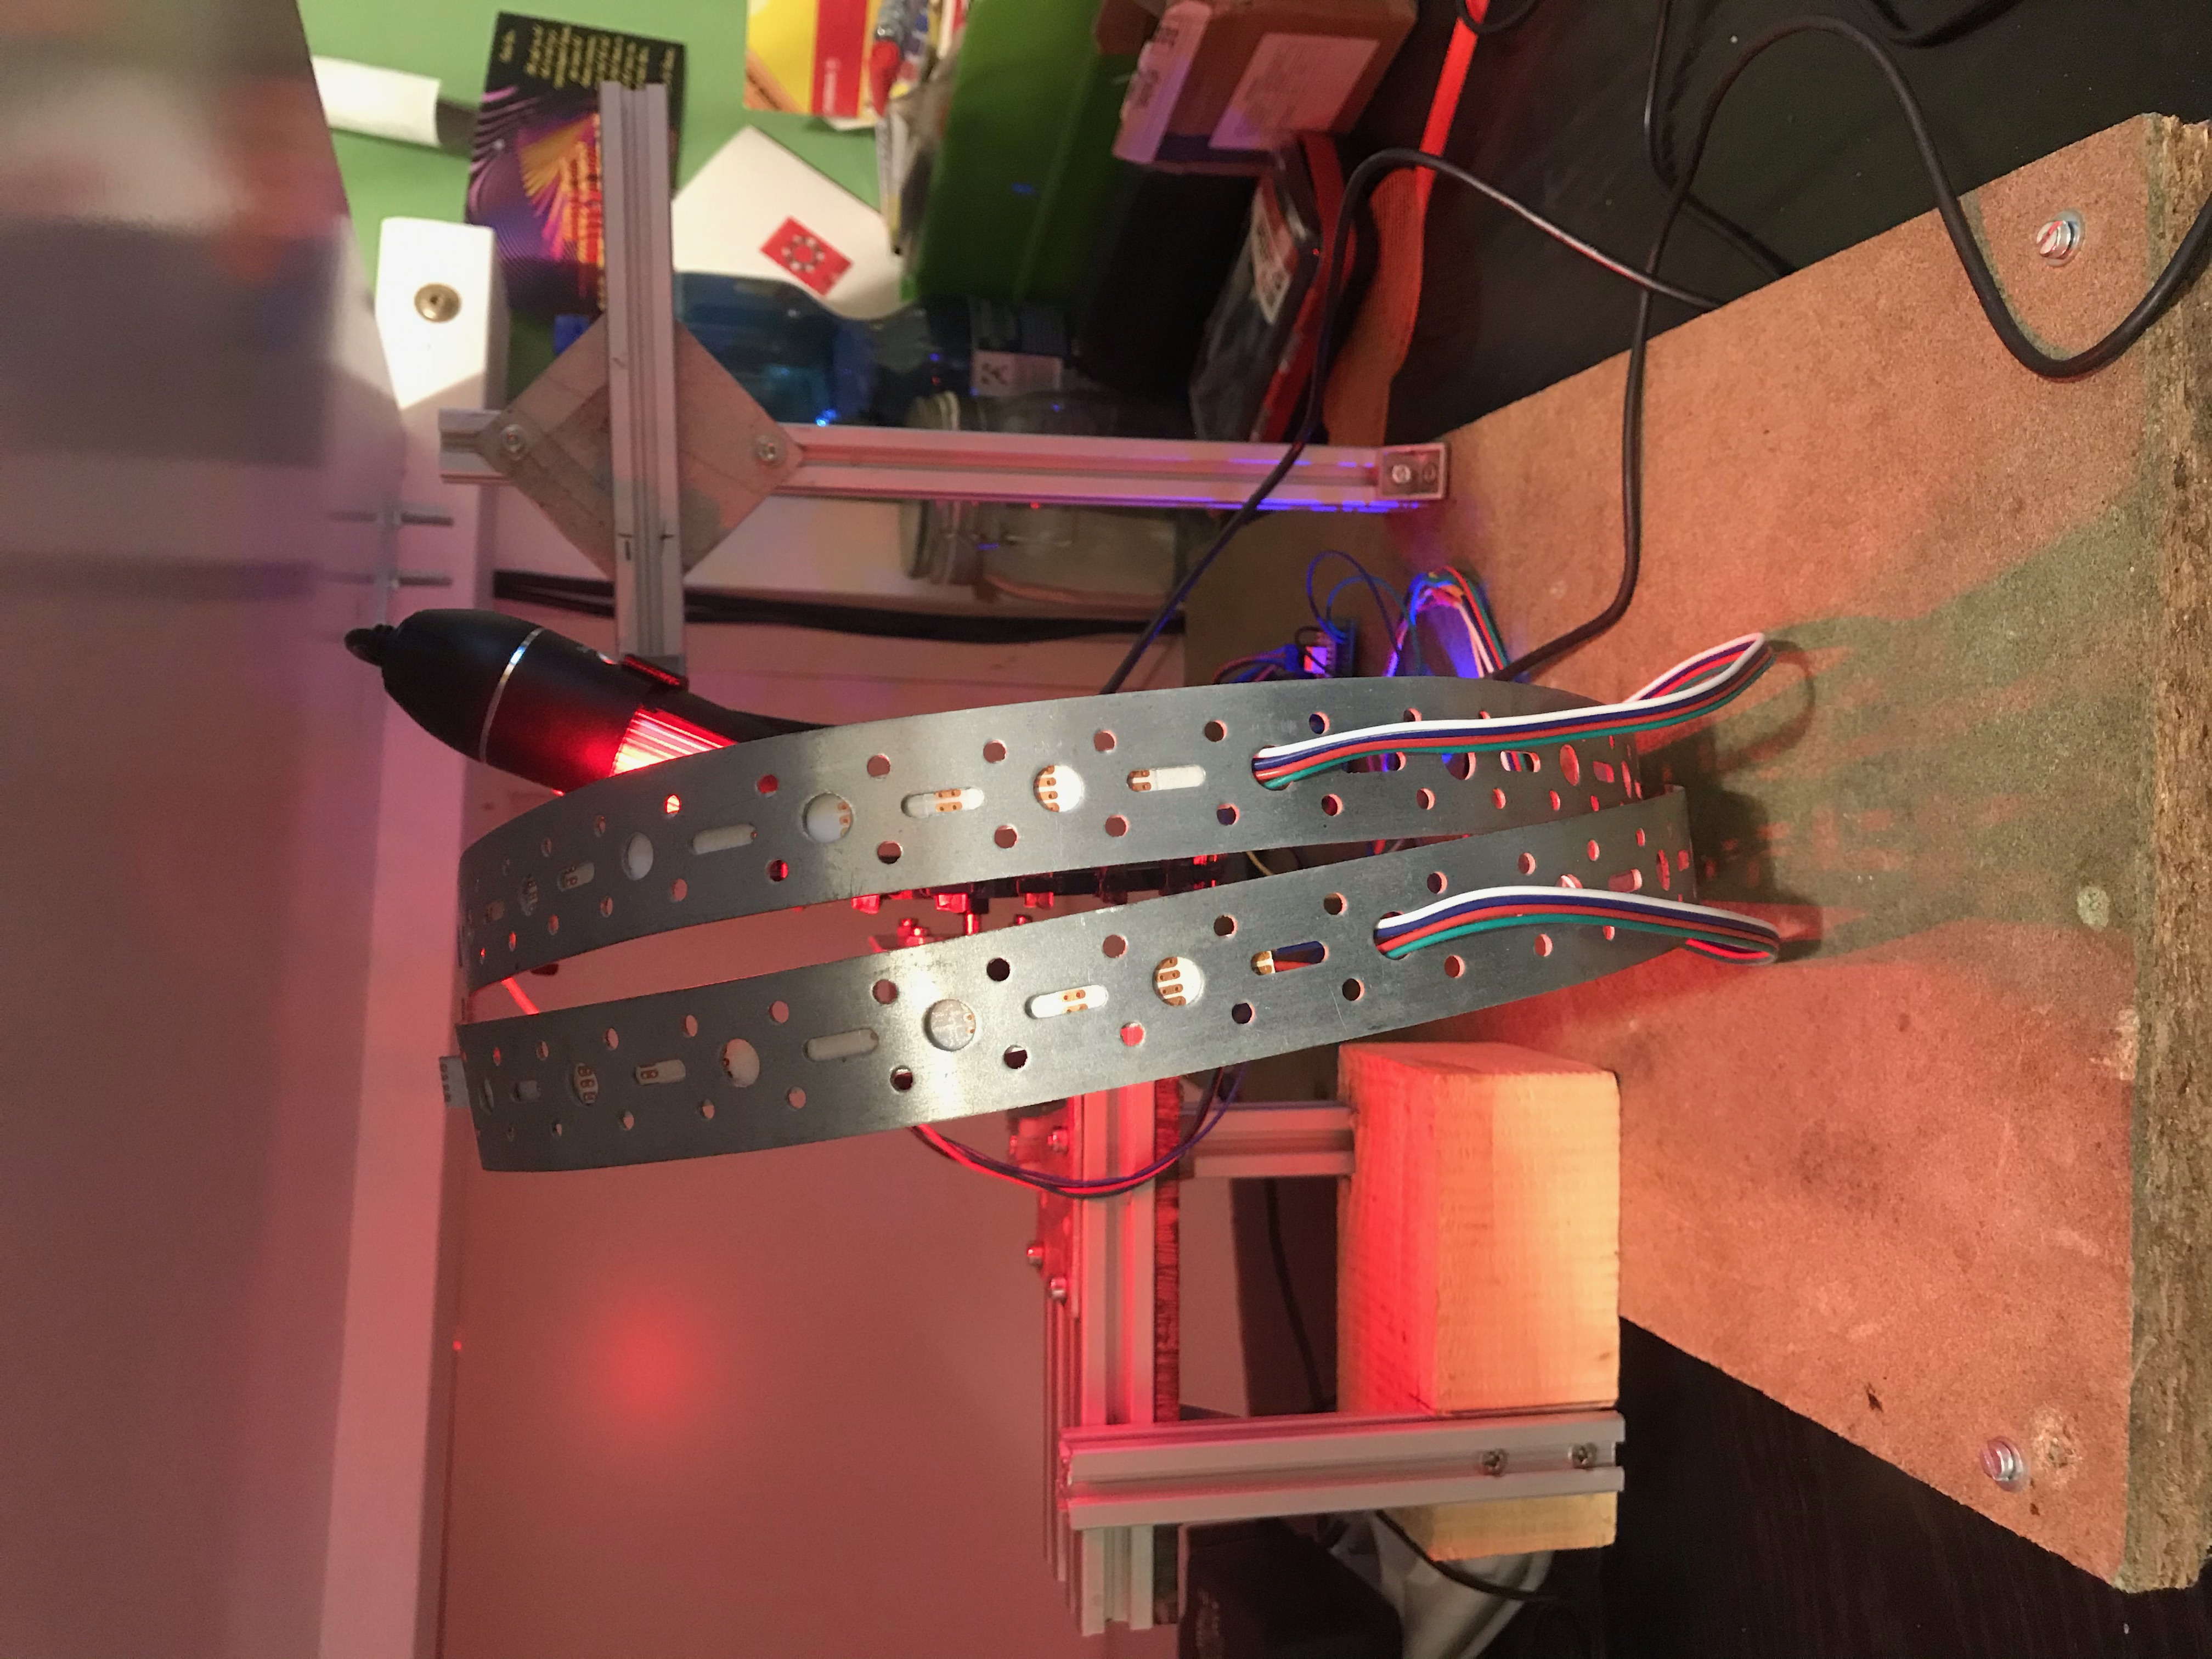
\includegraphics[width=4.166667in, keepaspectratio=true]{./2_Spaghetti_dataset/IMG_9295.jpeg}



The camera angle is kept the same a little to the top and very close to the inserts as seen on the next picture:

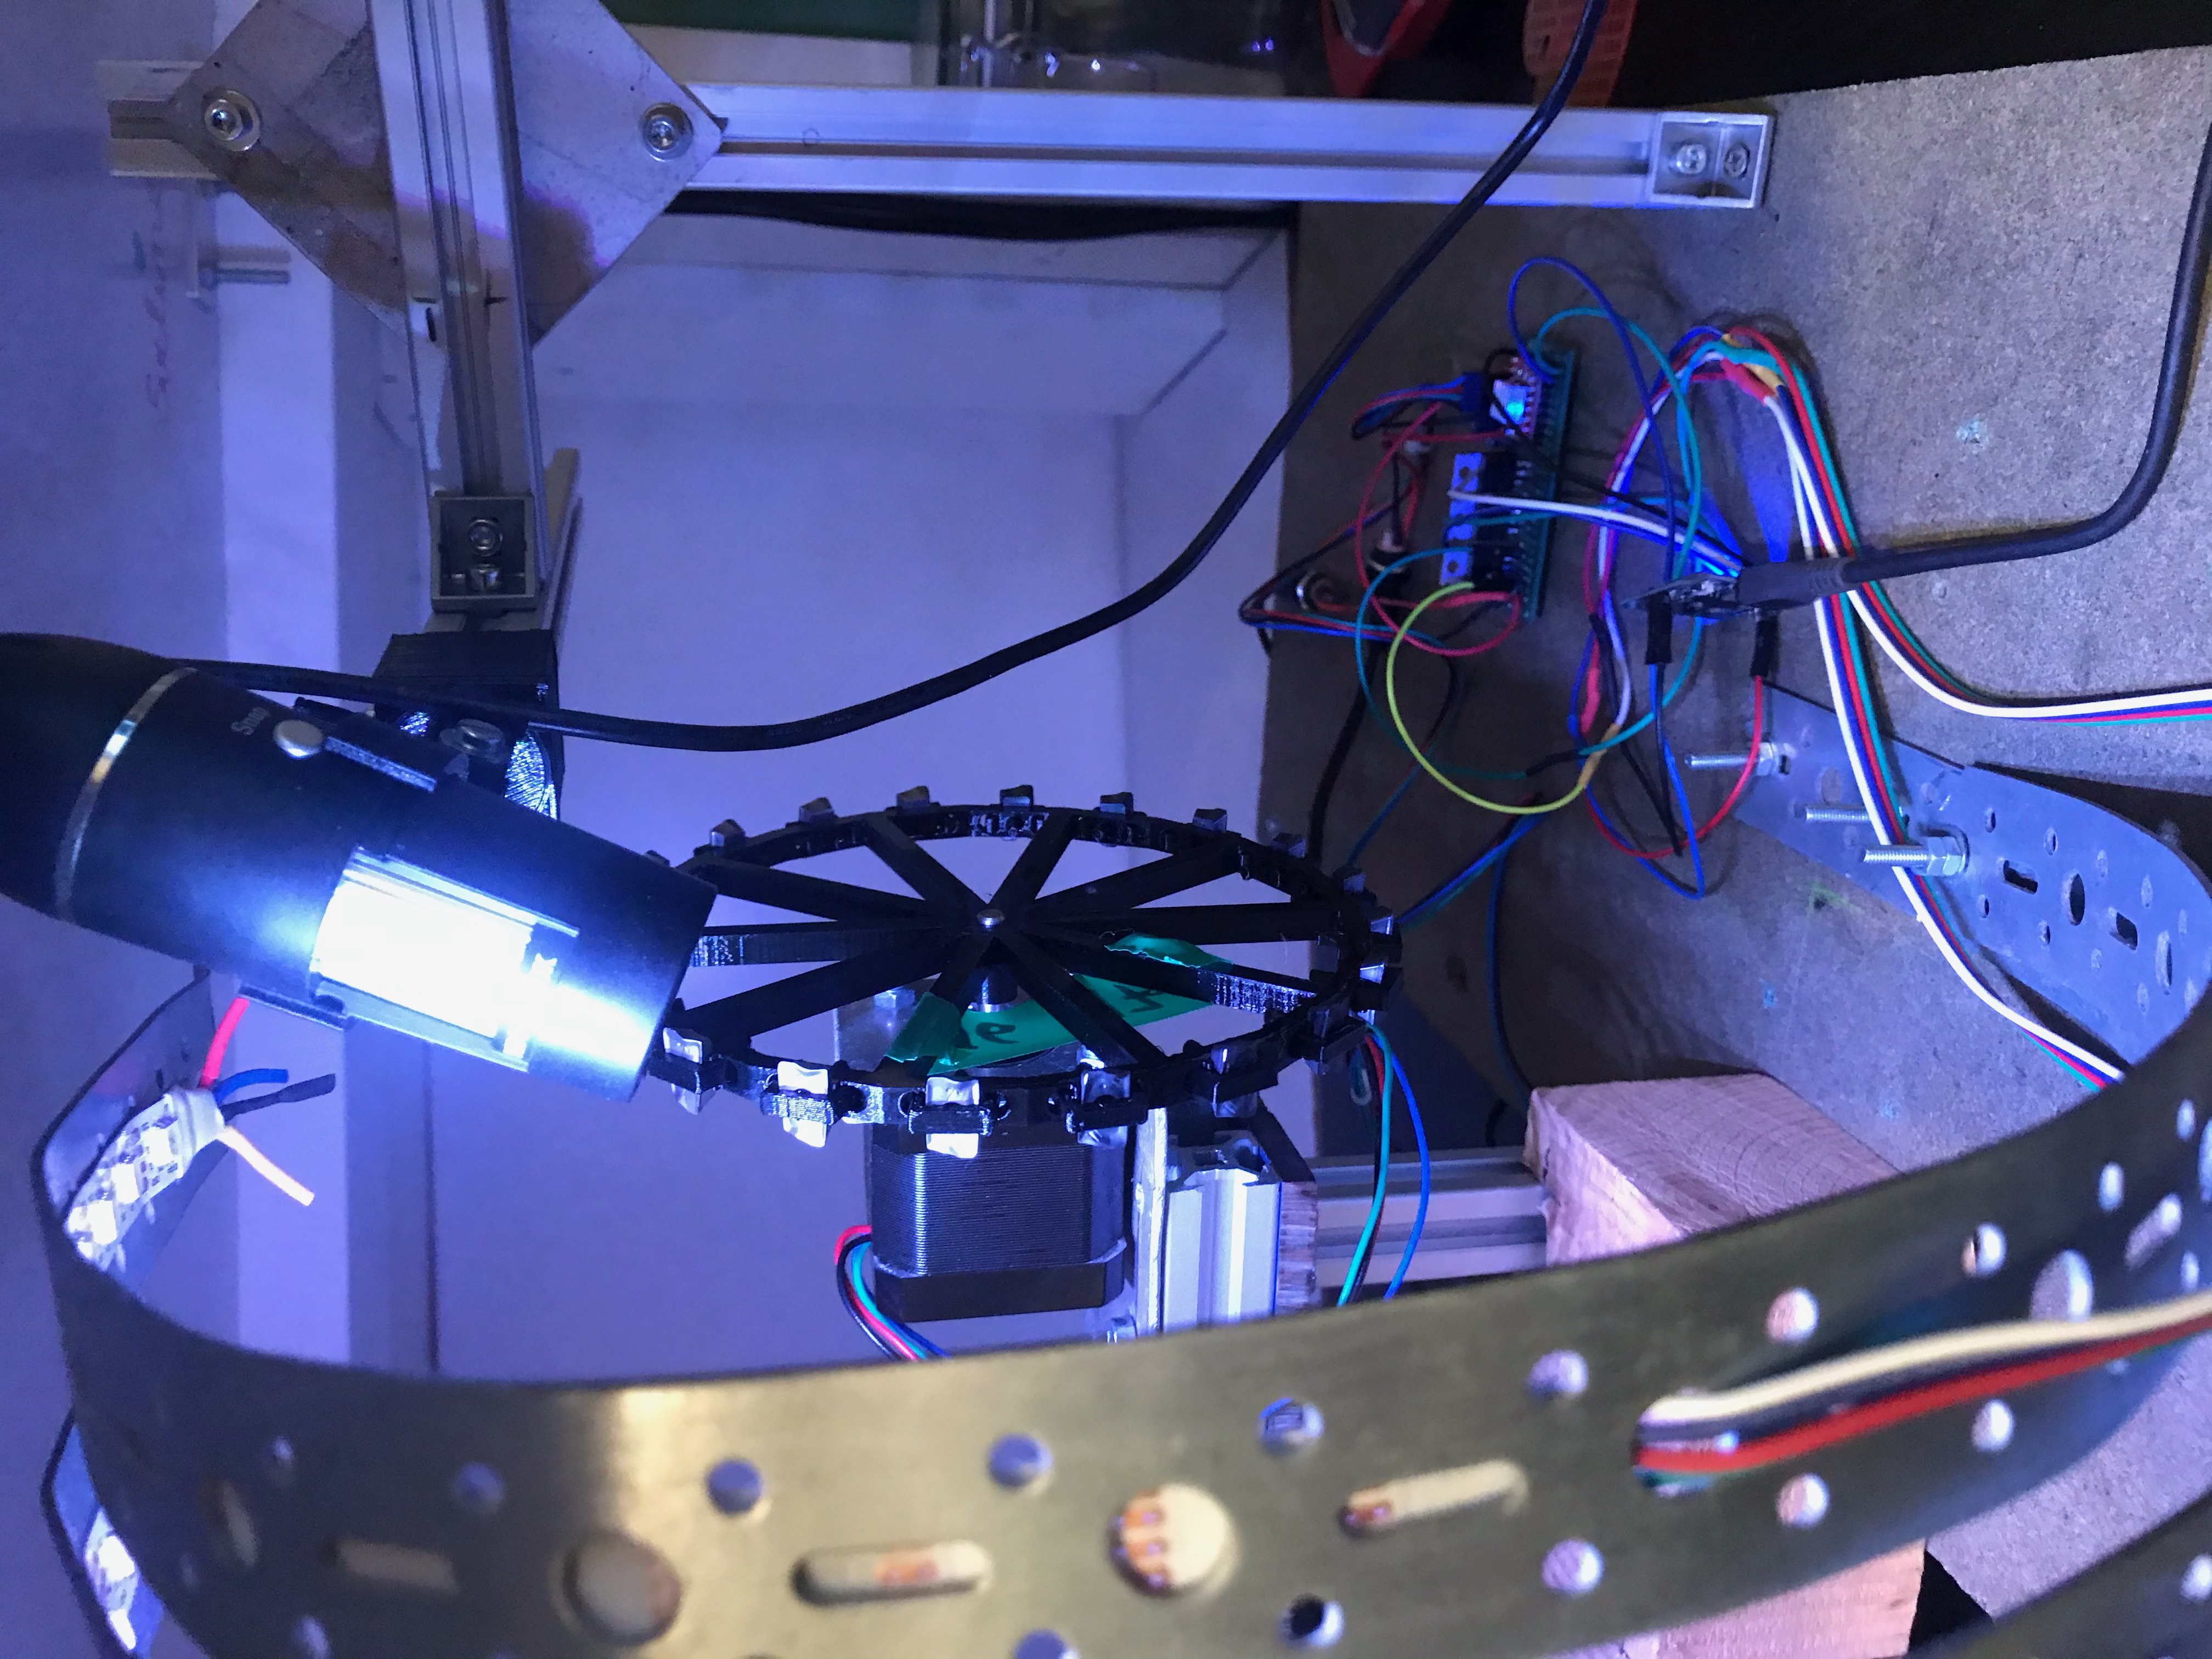
\includegraphics[width=4.166667in, keepaspectratio=true]{./2_Spaghetti_dataset/IMG_9296.jpeg}



Through the whole dataset the direct light coming from other sources eg. the light of the room was blocked to have full control of the lighting conditions.



\subsection{Results}

Underneath are some pictures of good examples in the dataset.



Underneath are two pictures of batch 3 insert 6. These where lid with red light on the left and white light on the right. Here is a nice wear shown and lighted. However if we zoom in to the picture the top part of the wear is not lighted that well. We can also see a white piece of the insert holder on the image which is providing som extra difficulties. The discussion of these difficulties will be bespoken in \href{../../../../Research/Vision_Algorithm.tex}{vision algorithm.}

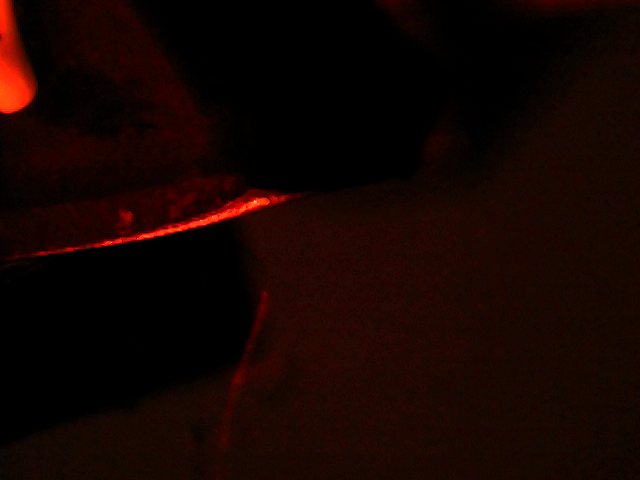
\includegraphics[width=3.125000in, keepaspectratio=true]{./2_Spaghetti_dataset/b_003_p_006_l_006-011_red_nb.png}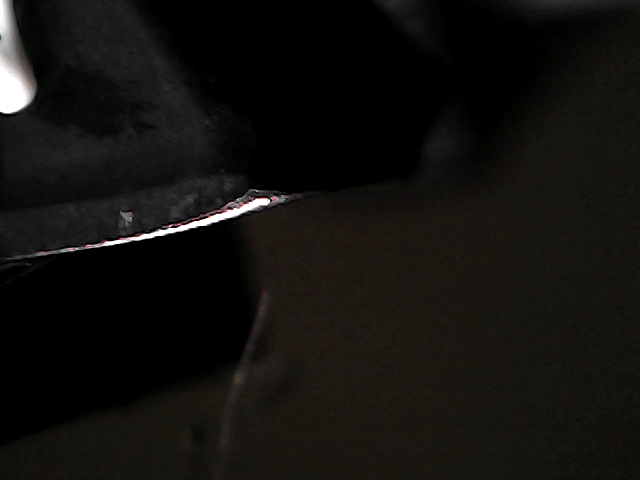
\includegraphics[width=3.125000in, keepaspectratio=true]{./2_Spaghetti_dataset/b_003_p_006_l_006-011_white_nb.png}



Some pictures aren't sharp like the one shown next.

like batch 5 insert 5 withoud bullet.

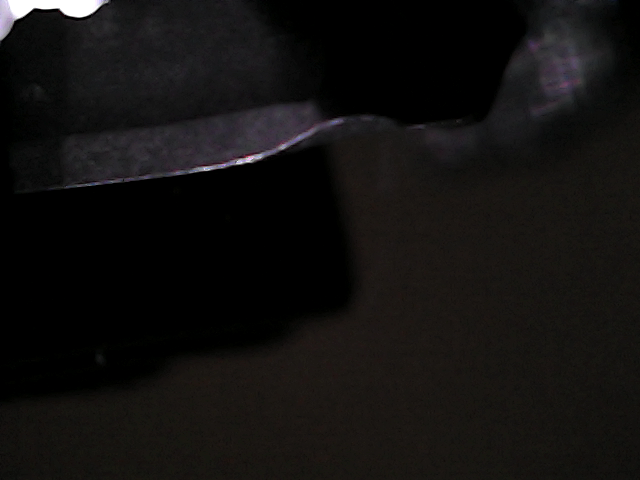
\includegraphics[width=3.125000in, keepaspectratio=true]{./2_Spaghetti_dataset/b_005_p_005_l_006-011_white_nb.png}



\paragraph{Different insert types}

First type are the grey inserts with very visible wear. These are seen in batches 1 to 5 consistently. This type will be called grey inserts.

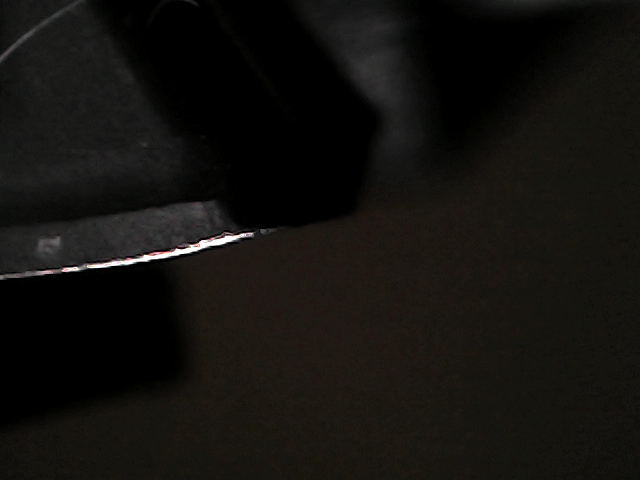
\includegraphics[width=3.125000in, keepaspectratio=true]{./2_Spaghetti_dataset/gray_b_003_p_004_l_006-011_white_nb.png}



Than there are other inserts in batch 11 which are also grey but have a different shape on the cutting part. These will be called rounded grey inserts.

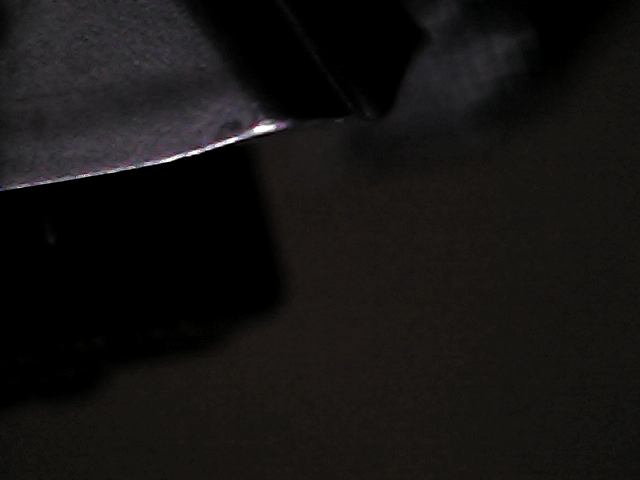
\includegraphics[width=3.125000in, keepaspectratio=true]{./2_Spaghetti_dataset/rounded_grey_b_011_p_008_l_006-011_white_nb.png}

In batch 12 and 13 there are the same shape of inserts but with a black coating which results in way darker pictures as seen here on batch 13 insert 2 no bullet. These inserts are the rounded black inserts.

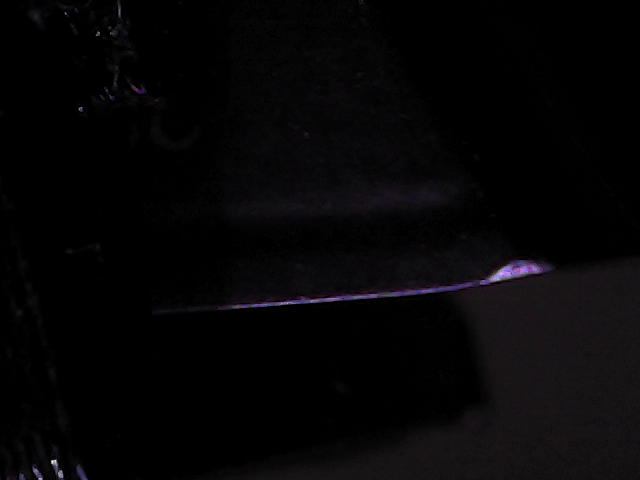
\includegraphics[width=3.125000in, keepaspectratio=true]{./2_Spaghetti_dataset/rounded_black_b_013_p_002_l_006-011_white_nb.png}



The next type are copper colored inserts with the rounded shape. Seen in batch 14 insert 5 no bullet.

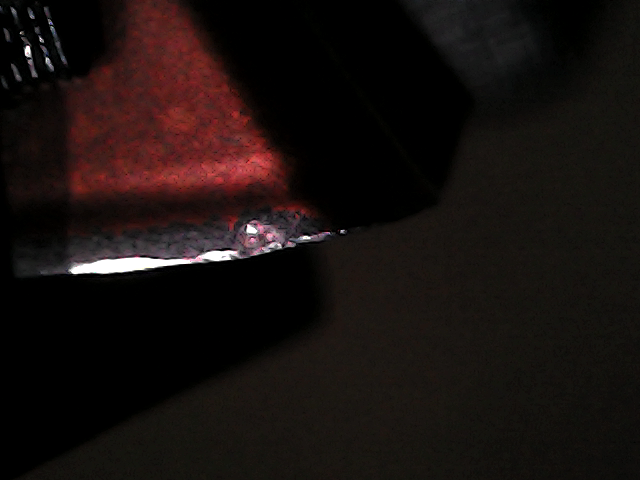
\includegraphics[width=3.125000in, keepaspectratio=true]{./2_Spaghetti_dataset/rounded_copper_b_014_p_005_l_006-011_white_nb.png}



Than we have inserts with a gold coating and hooked shape. For batch 15 insert 6 no bullet that gives the next picture:

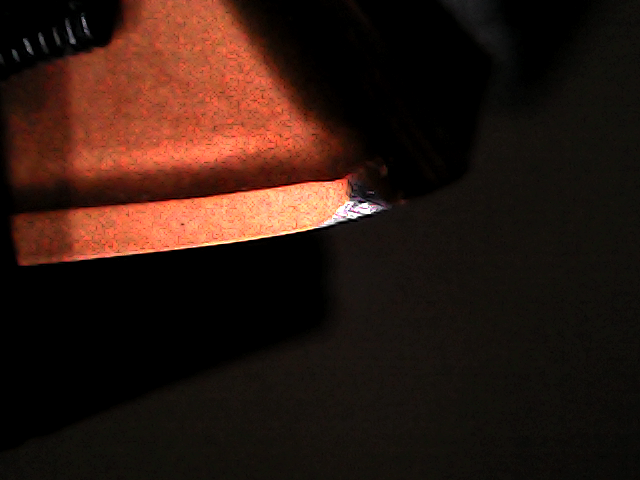
\includegraphics[width=3.125000in, keepaspectratio=true]{./2_Spaghetti_dataset/rounded_gold_b_015_p_006_l_006-011_white_nb.png}





































\end{document}
